\documentclass{beamer}
\usepackage{header/packages}

%gets rid of bottom navigation symbols
%\setbeamertemplate{navigation symbols}{}

%gets rid of footer
%will override 'frame number' instruction above
%comment out to revert to previous/default definitions
%\setbeamertemplate{footline}{}

% Tác giả, Tiêu đề, vân vân
\title[]{{\huge \bf Graduation Thesis} \\
\large Run length limited de Bruijn sequences for quantum communication}
% \author[Nguyen Tien Long]{
% Nguyen Tien Long, CTTN-CNTT-K63% \inst{1} 
% \\ {\small Supervisors: supervisor1 \\ \hspace{18mm} supervisor2}

% }

\author[Nguyen Tien Long]{
Nguyen Tien Long
\texorpdfstring{ \\ {\small Supervisors: Dr. Vu Van Khu}  \\ {\small \hspace{21mm} Dr. Tran Vinh Duc}}{}
}
% \author[Supervisors]{ {\small Supervisors: Dr. Vu Van Khu}  \\ {\small \hspace{22mm} Dr. Tran Vinh Duc}}

\institute[]{
%\inst{1}% 
School of Information and Communication Technology.
}

\date{August 18, 2022}


% \logo{
\includegraphics[scale=0.05]{BVP-logo bk-rgb.jpg} \vspace{220pt}}
\logo{
    \begin{tikzpicture}[overlay,remember picture]
    \node[left=0.05cm] at (current page.-33){
        
\includegraphics[scale=0.04]{BVP-logo bk-rgb.jpg}
    };
    \end{tikzpicture}
}
\pgfplotsset{compat=1.18}
\begin{document}

\begin{frame}
    \titlepage
\end{frame}

\begin{frame}
    \frametitle{Table of Contents}
    \tableofcontents
\end{frame}

% \section{Introduction}
% \begin{frame}{Coding Theory}
    \begin{itemize}
        \item The study of the properties of codes and their respective fitness for specific applications.
    \end{itemize}
    \begin{columns}
        \begin{column}{0.5\textwidth}
            \begin{figure}
            \centering
                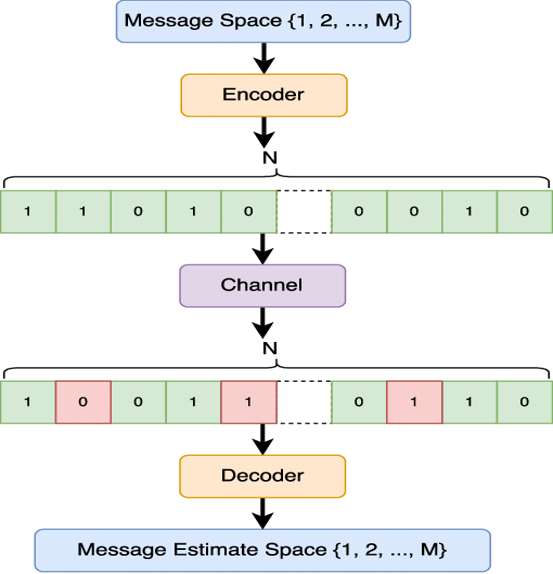
\includegraphics[width=0.8\textwidth]{Images/Introduction/CodingTheory.png}
                \caption{Coding Process.}
                \label{fig:coding_process}
            \end{figure}
        \end{column}
        
        \begin{column}{0.5\textwidth}
            \begin{figure}
                \centering
                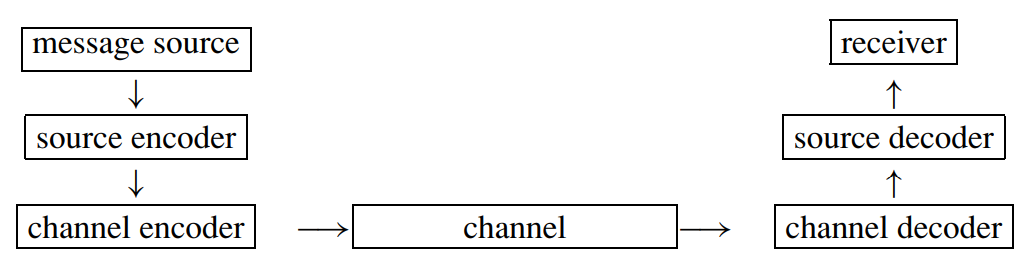
\includegraphics[width=\textwidth]{Images/Introduction/sourceandchannelcoding.png}
                \caption{Source and Channel Coding.}
                \label{fig:sourcechannelcoding}
            \end{figure}    
        \end{column}    
    \end{columns}
\end{frame}

\begin{frame}{Coding Theory - Applications}
    \begin{columns}
        \begin{column}{0.5\textwidth}
            \begin{itemize}
                \vfill \item Run length limited code is used in CD, DVD.
                \begin{figure}
                    \centering
                    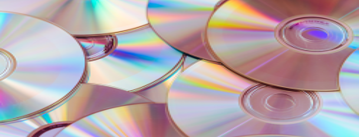
\includegraphics[width=0.7\textwidth]{Images/Introduction/CDDVD.png}
                    % \caption{Caption}
                    % \label{fig:my_label}
                \end{figure}
                \hfill
                \vfill \item 3G,4G networks use Reed- Solomon code.
                \begin{figure}
                    \centering
                    
\includegraphics[width=0.7\textwidth]{Images/Introduction/3G4G.png}
                    % \caption{Caption}
                    % \label{fig:my_label}
                \end{figure}
                \vfill \item 5G networks use Turbo code.
                \begin{figure}
                    \centering
                    
\includegraphics[width=0.7\textwidth]{Images/Introduction/5G.png}
                    % \caption{Caption}
                    % \label{fig:my_label}
                \end{figure}
            \end{itemize}
        \end{column}
        
        \begin{column}{0.5\textwidth}
            \begin{itemize}
                \vfill \item LDPC code is used in Data modems, telephone transmissions, and the NASA Deep Space Network.
                \begin{figure}
                    \centering
                    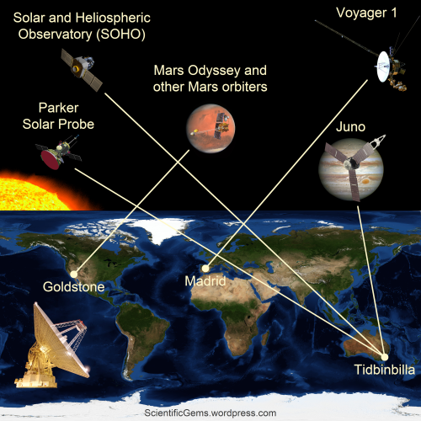
\includegraphics[width=0.8\textwidth,height=0.6\textheight]{Images/Introduction/NASA.png}
                    % \caption{Caption}
                    % \label{fig:my_label}
                \end{figure}
            \end{itemize}
        \end{column}
    \end{columns}
\end{frame}


\begin{frame}{Constrained Code}
    \begin{itemize}
        \vfill \item Code: set of (binary) sequences, strings.
        
        $\rightarrow$ Constrained code $\mathbb{C}$: set of sequences satisfying given constraints.
        \vfill \item Presentation: a directed graph $G=(V,E)$.
        \vfill \item Path: sequence of edges $\left(e_{1},e_{2},\ldots,e_{n}\right)$ such that the end vertex of $e_{i}$ is the start vertex of $e_{i+1}$ $e_{i}\in E$. 
        \vfill \item Simple path: path with no repeated edges.
    \end{itemize}
\end{frame}

\begin{frame}{De Bruijn Code (Positioning Code)}
    \begin{columns}
        \begin{column}{0.65\textwidth}
            \begin{enumerate}
                \item De Bruijn graph of order $k$, $G_{k}$:
                \begin{itemize}
                    \item Each vertex is labeled by a sequence of length $k-1$.
                    \item A directed edge from $\bfx = \left[x_{0}x_{1}\ldots x_{k-2}\right]$ to $\bfy=\left[y_{0}y_{1}\ldots y_{k-2}\right]$ $\Leftrightarrow\ x_{1}x_{2}\ldots x_{k-2}=y_{0}y_{1}\ldots y_{k-3}$. 
                \end{itemize}
                \item De Bruijn sequence:
                \begin{itemize}
                    \item A cyclic binary de Bruijn of order $k$ is a length $2^{k}$ sequence such that each length $k$ string appears exactly once.
                    \item Longest simple path in de Bruijn graph (Eulerian cycle) $\equiv$ de Bruijn sequence.
                \end{itemize}
                
                \item Applications:
                \begin{itemize}
                    \item Cryptography.
                    \item Interconnection networks.
                    \item VLSI testing.
                    \item Combine with biology: DNA storage.
                \end{itemize}
            \end{enumerate}
        \end{column}
        
        \begin{column}{0.35\textwidth}
            \begin{figure}
                \centering
                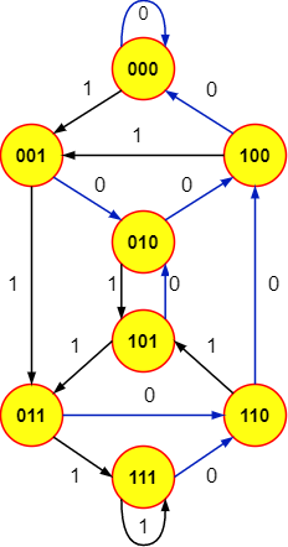
\includegraphics[width=0.8\textwidth]{Images/deBruijnOrder4.png}
                \caption{de Bruijn graph of order $4$.}
                \label{fig:dB4}
            \end{figure}
        \end{column}
    \end{columns}
\end{frame}

\begin{frame}{What do we concern about a code?}
    \begin{block}<1>{Rate}
        Rate and Maximal asymptotic rate tend to as high as possible.
    \end{block}
    \begin{block}<1>{Efficient encoding algorithm}
        Encoding algorithm: maps messages into codewords, generates sequences in the code, \dots.
    \end{block}
    \begin{block}<1>{Efficient decoding algorithm}
        Decoding algorithm: maps codewords into messages, locates the position of the sequences in the ordered code, \dots.
    \end{block}
    \begin{block}<0>{Et Cetera}
        Fault tolerant, robust positioning, \dots.
    \end{block}
\end{frame}

\section{Introduction}
\begin{frame}{Satellite Quantum Key Distribution (QKD)}
    \visible<1->{
        Quantum Key Distribution.
        % \begin{itemize}
        %     \item Cryptographic protocol involving components of quantum mechanics.
        %     \item Enables two parties to produce a shared random secret key known only to them.
        % \end{itemize}
    }
    
    \begin{overprint}
        \onslide<1>
        \begin{itemize}
            \item Cryptographic protocol involving components of quantum mechanics.
            \item Enables two parties to produce a shared random secret key known only to them.
        \end{itemize}
        \onslide<2->
        Satellite QKD: share random key between satellite and ground station.
        \visible<3->{
        
        A classical channel is used along to synchronise quantum channel~\sfcite{zhang2021timing,khader2018time}.
        \begin{figure}
            \centering
            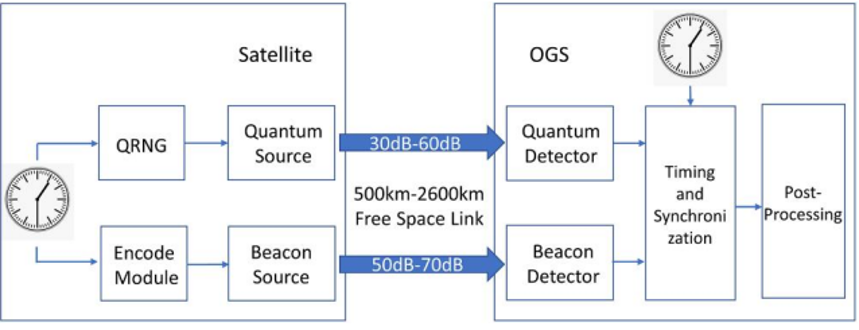
\includegraphics[scale=.3]{Images/Motivation/SatteliteQKD.png}
            \caption{High-level satellite Quantum Key Distribution schematic~\sfcite{zhang2021timing}.}
            \label{fig:satelliteQKD}
        \end{figure}
    }    
    \end{overprint}
    
    % \visible<2->{
    %     Satellite QKD: share random key between satellite and ground station
        
    % }
    
    % \visible<3->{
    %     A classical channel is used along to synchronise quantum channel~\sfcite{duan2021survey,khader2018time}.
    %     \begin{figure}
    %         \centering
    %         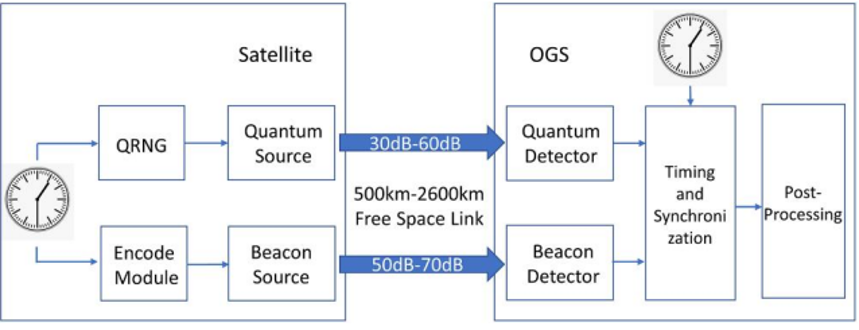
\includegraphics[scale=.3]{Images/Motivation/SatteliteQKD.png}
    %         \caption{High-level satellite Quantum Key Distribution schematic.}
    %         \label{fig:satelliteQKD}
    %     \end{figure}
    % }
\end{frame}

% \begin{frame}{Satellite Quantum Key Distribution (QKD)}
%     Commercial QKD: deployed over optical fibre.
%     \begin{overprint}
%         \onslide<1>
%         But: $$\mathrm{range}< 1000 \mathrm{km}$$
%         \onslide<2>
%         But: $$\mathrm{range}< 1000 \mathrm{km}$$
%         $\rightarrow$ Satellite QKD: alternative method to establishing intercontinental secure communication links.
        
%         \onslide<3> 
%         But: $$\mathrm{range}< 1000 \mathrm{km}$$
%         $\rightarrow$ Satellite QKD: alternative method to establishing intercontinental secure communication links.
        
%         Challenges:
%         \begin{itemize}
%             \item High channel losses.
%             \item Rapid relative motion between the transmitter and receiver.
%         \end{itemize}
%         \onslide<4-> 
%         % \visible<4->{
%         $\rightarrow$ Satellite QKD: alternative method to establishing intercontinental secure communication links.
        
%         $\rightarrow$ A classical channel is used along to synchronise quantum channel~\sfcite{duan2021survey,khader2018time}.
%         \begin{figure}
%             \centering
%             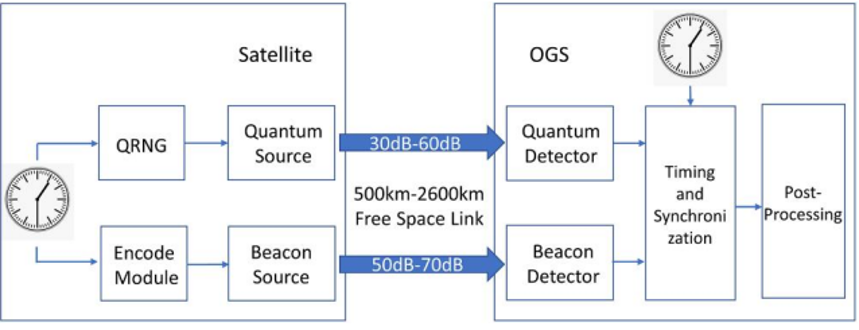
\includegraphics[scale=.3]{Images/Motivation/SatteliteQKD.png}
%             \caption{High-level satellite Quantum Key Distribution schematic.}
%             \label{fig:satelliteQKD}
%         \end{figure}
%         % }
%     \end{overprint}
    
%     % \visible<3->{
%     %     $\Rightarrow$ A classical channel is used along to synchronise quantum channel~\sfcite{duan2021survey,khader2018time}.
%     %     \begin{figure}
%     %         \centering
%     %         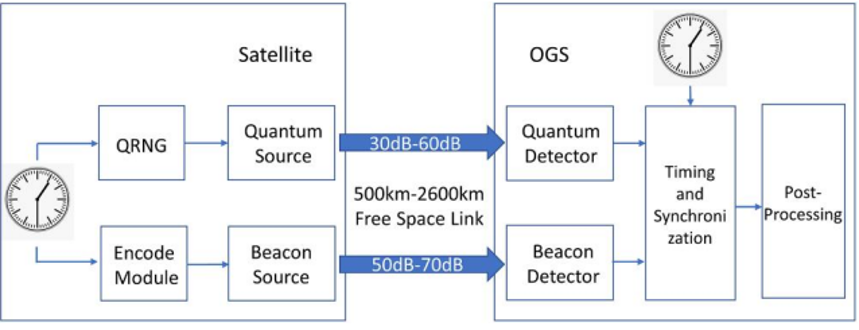
\includegraphics[scale=.3]{Images/Motivation/SatteliteQKD.png}
%     %         \caption{High-level satellite Quantum Key Distribution schematic.}
%     %         \label{fig:satelliteQKD}
%     %     \end{figure}
%     % }
% \end{frame}


\begin{frame}{Related Work}
    \citeauthor{zhang2021timing}\sfcite{zhang2021timing}: de Bruijn based timing-synchronization system (dBTS).
    \begin{overprint}
        \onslide<2-4> 
            \begin{columns}
            \visible<2->{
                \begin{column}{.37\textwidth}
                    \begin{centering}
                        \fcolorbox{red}{white}{Encode}
                        \begin{figure}
                            % \centering
                            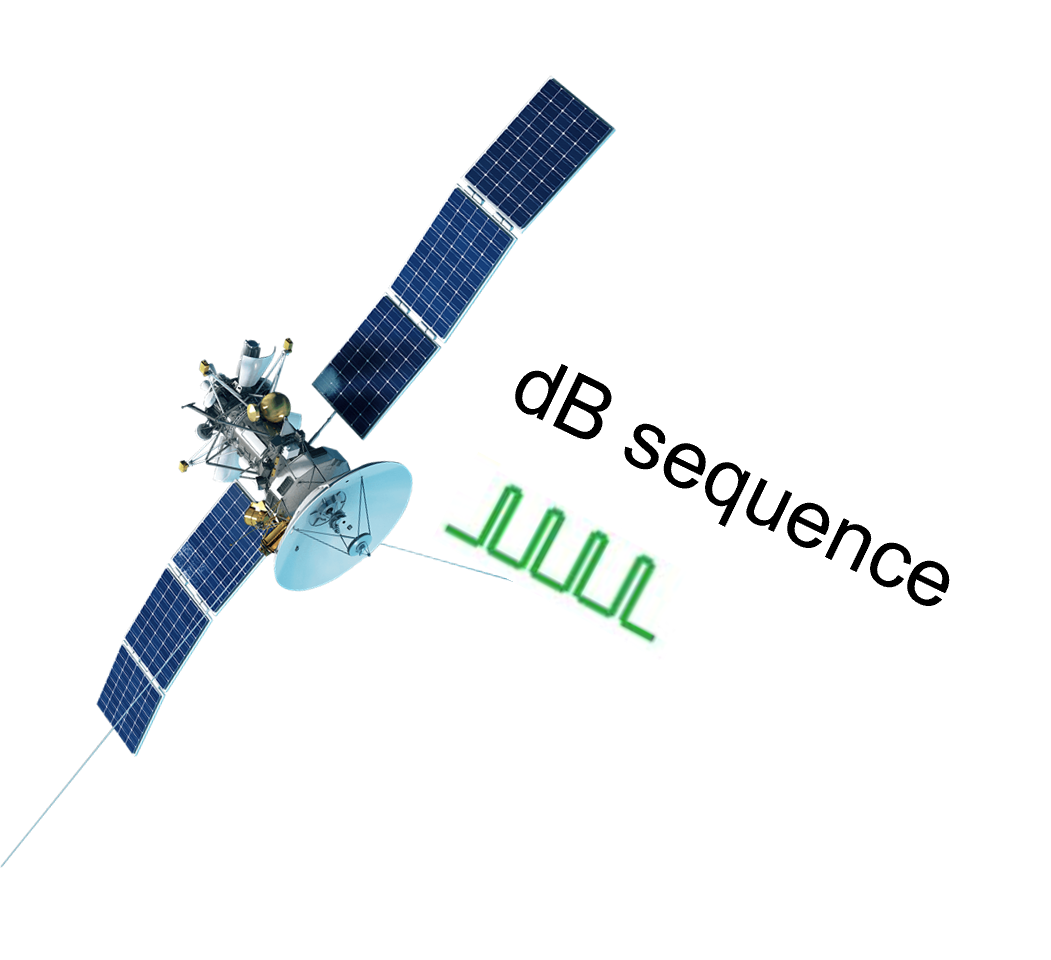
\includegraphics[width=0.6\textwidth]{Images/Motivation/SatelliteEncode.png}
                            % \caption{Caption}
                            % \label{fig:my_label}
                        \end{figure}
                    \end{centering}
                    \begin{itemize}
                        \item Linear feedback shift register (LFSR): generate an order $k$ de Bruijn sequence.
                    \end{itemize}
                \end{column}
                \vrule{}
            }
            \visible<3->{
                \begin{column}{.26\textwidth}
                    \begin{centering}
                        \fcolorbox{red}{white}{Noisy channel}
                        \begin{figure}
                            % \centering
                            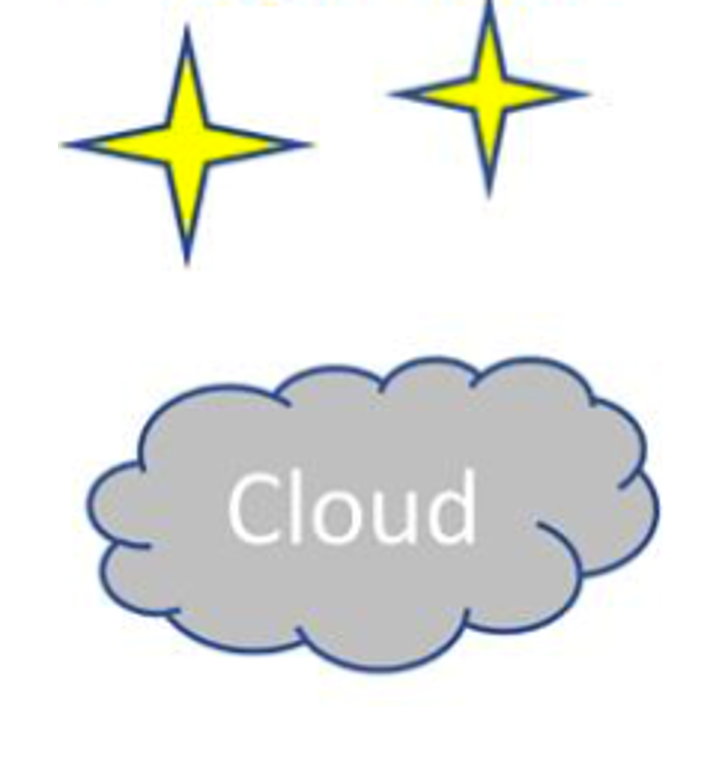
\includegraphics[width=0.6\textwidth]{Images/Motivation/Cloud.png}
                            % \caption{Caption}
                            % \label{fig:my_label}
                        \end{figure}
                    \end{centering}
                \end{column}
                \vrule{}
            }
            \visible<4->{
                \begin{column}{.37\textwidth}
                    \begin{centering}
                        \fcolorbox{red}{white}{Decode}
                        \begin{figure}
                            % \centering
                            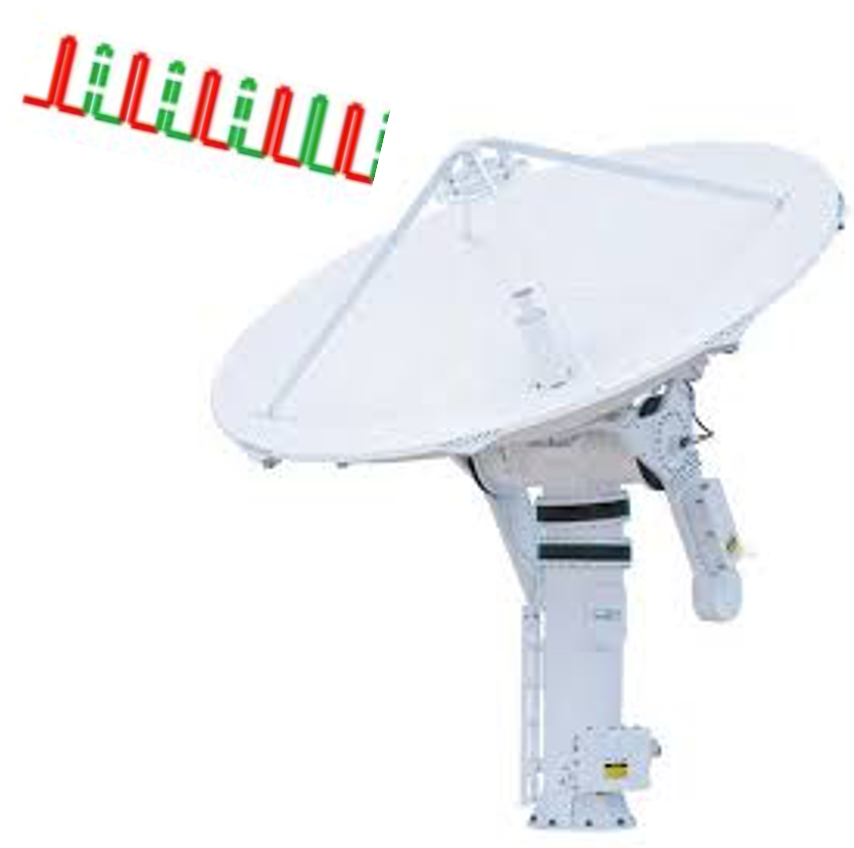
\includegraphics[width=0.5\textwidth]{Images/Motivation/GSDecode.png}
                            % \caption{Caption}
                            % \label{fig:my_label}
                        \end{figure}
                    \end{centering}
                    \begin{itemize}
                        \item Look-up table: locate the position of a length $k$ subsequence in the whole sequence.
                    \end{itemize}
                \end{column}
            }
            \end{columns}
        \onslide<5->
            \visible<5->{
                \begin{block}{Transmit a modulated sequence}
                    \begin{itemize}
                        \item {\color{red}Constraint}: avoid long period of no pulse .
                        \item {\color{red}Requirement}: positioning sequence.
                        \item {\color{red}Method}: de Bruijn sequence, pulse modulation: $1\rightarrow\mathrm{on-on},\ 0\rightarrow\mathrm{on-off}$, called Hybrid de Bruijn (HdB) sequence.
                    \end{itemize}
                \end{block}
            }
            \visible<6->{
                \begin{alertblock}{Drawback}
                    \begin{itemize}
                        \item $\mathrm{Rate}=0.5$.
                        \item Encode: LFSR (prerequisite: suitable primitive polynomial).
                        \item Decode: use look-up table (exponential complexity).
                    \end{itemize}
                \end{alertblock}
            }
    \end{overprint}
    
\end{frame}

\begin{frame}{Contributions}
    \begin{block}{Propose a new combinatorial object RdB}
        \begin{itemize}
            \item Can be encoded and decoded efficiently.
            \item Can replace HdB sequence: higher rate and maximal asymptotic rate, more general and adaptive.
        \end{itemize}
    \end{block}
    \begin{block}{Determine the maximal length of RdB}
        \begin{itemize}
            \item Explicit formula.
        \end{itemize}
    \end{block}
    \begin{block}{Encoding and Decoding Algorithm}
        \begin{itemize}
            \item Encoder: Constant amortized time per symbol.
            \item Decoder: Sub-linear time with respect to the length of the sequence.
        \end{itemize}
    \end{block}
\end{frame} 



\section{Run length limited de Bruijn sequences}
\begin{frame}{Run Length Limited de Bruijn (RdB) code}
    \begin{definition}
        A $(k,s)$-RdB sequence: a de Bruijn sequence of order $k$ containing at most $s$ consecutive bit $0$'s.
    \end{definition}
    \begin{overprint}
        \onslide<1> 
            Trivial cases:
            \begin{itemize}
                \item $s\geq k$: original de Bruijn sequence.
                \item $s=k-1$: remove $0^k-1$ in the de Bruijn graph.
            \end{itemize}
            $\Rightarrow$ Interested in:
            \begin{itemize}
                \item $s<k-1$: eliminate vertices with more than $s$ consecutive bit $0$'s.
            \end{itemize}
        \onslide<2->
            \begin{columns}
            \visible<2->{
                \begin{column}{0.33\textwidth}
                    \begin{figure}[htbp]
                        \centering
                        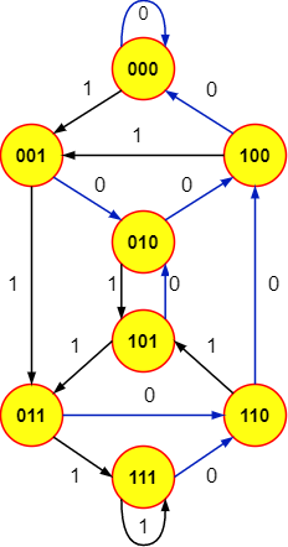
\includegraphics[scale=0.27]{Images/deBruijnOrder4.png}
                        \caption{de Bruijn graph of order $4$.}
                        % \label{fig:my_label}
                    \end{figure}
                \end{column}
            }
            \visible<3->{
                \begin{column}{0.33\textwidth}
                    \begin{figure}[htbp]
                        \centering
                        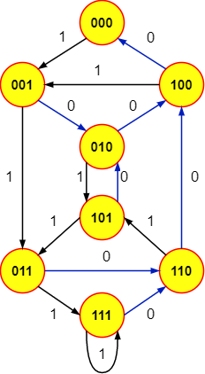
\includegraphics[scale=0.35]{Images/RdB/RdB_4_3.png}
                        \caption{$(4,3)$-RdB graph.}
                        \label{fig:RdB_4_3}
                    \end{figure}
                \end{column}
            }
            \visible<4->{
                \begin{column}{0.34\textwidth}
                    \begin{figure}[htbp]
                        \centering
                        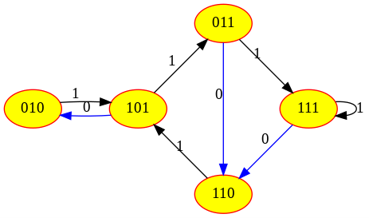
\includegraphics[scale=0.4]{Images/RdB/RdB_4_1.png}
                        \caption{$(4,1)$-RdB graph.}
                        \label{fig:RdB_4_1}
                    \end{figure}
                \end{column}
            }
        \end{columns}
    \end{overprint}
    
    
\end{frame}

\begin{frame}{Maximal length of $(k,s)$-RdB sequence}
    Given $k,s$. Notations:
    \begin{itemize}
        \item $\ell(k,s)$: maximal length of simple path $(k,s)$-RdB graph.
        \item $N(k,s)$: maximal length of $(k,s)$-RdB sequences $(=\ell(k,s)+k-1)$.
    \end{itemize}
    \begin{theorem}
        Given $k,s$. Then:
        \begin{align}
            \ell(k,s) = \card{W(k,s)} - \left(\sum_{i=0}^{C}(s-i)\card{W(k-s-i-3,s)}-s\right)
        \end{align}
    \end{theorem}
    where :
    \begin{itemize}
        \item $C=\min(s-1,k-s-2)$.
        \item $W(n,s)$: set of length $n$ sequences containing at most $s$ consecutive bit $0$'s. 
    \end{itemize}
\end{frame}

\begin{frame}{Maximal length of $(k,s)$-RdB sequence}
    \begin{lemma}
        \centering
        $\ell(k,s)\leq\card{W(k,s)} - \left(\sum_{i=0}^{C}(s-i)\card{W(k-s-i-3,s)}-s\right) $
    \end{lemma}
    Observe:
    \begin{itemize}
        \item Vertices: balance, right-unbalanced, left-unbalanced.
        \item Number of left(right)-unbalanced vertices of form $0^{s}1\ldots10^{i}$ is $\card{W}(k-i-s-3,s)$ with $i\leq C=\min(s-1,k-s-2)$.
    \end{itemize}
    \begin{figure}
        \centering
        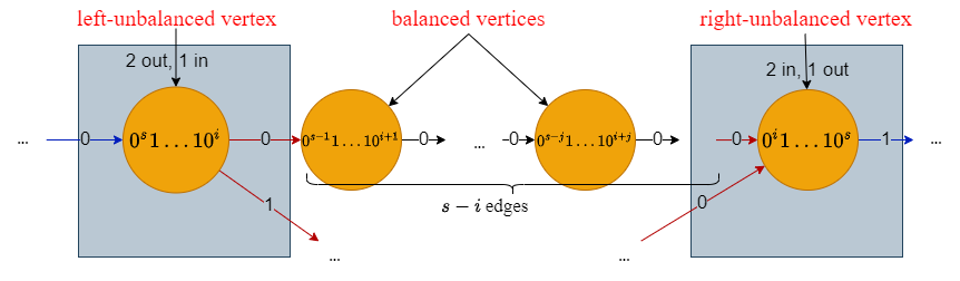
\includegraphics[width=0.9\textwidth,height=.3\textheight]{Images/Rate/sketchproof.png}
        \caption{Vertices in RdB graphs.}
        \label{fig:sketchproof}
    \end{figure}
\end{frame}

\section{Rate and Maximal Asymptotic Rate}
\begin{frame}{Definition of rate}
    Recall $N(k,s) = \ell(k,s)+k-1$. Given $k,s$:
    \begin{itemize}
        \item Let $\bfx_{k,s}$: a $(k,s)$-RdB sequence. The (information) rate of $\bfx_{k,s}$:
        \begin{align}
            R_{\bfx_{k,s}} = \dfrac{\log\left(\card{\bfx_{k,s}}\right)}{k}
        \end{align}
        \pause
        \item Maximal rate of $(k,s)$-RdB sequences:
        \begin{align}
            R_{k,s} = \dfrac{\log(N(k,s))}{k}
        \end{align}
        \pause
        \item  Maximal asymptotic rate of $(k,s)$-RdB sequences:
        \begin{align}
            R_{s} = \lim_{n\to\infty}\dfrac{\log(N(k,s))}{k}
        \end{align}
    \end{itemize}
\end{frame}

\begin{frame}{Maximal Asymptotic Rate}
    \begin{theorem}
        \centering $R_{1}= 0.6942$
    \end{theorem}
    which is larger than $0.5$, rate of HdB sequences.
    \begin{theorem}
        \begin{center}
            $R_{s} = \log(\card{\omega})$
        \end{center} 
        
        where $\omega$ is the root of equation: $x^{s+1}-x^{s}-\ldots-x-1=0$ such that $\card{\omega}$ is the largest.
    \end{theorem}
    \textit{Proof}: Approximation: $\card{W(k,s)}\approx a\card{\omega}^{n}$. Hence: 
    $$N(k,s)\approx \card{\omega}^{k-s-2}\left(\sum_{i=0}^{s}a(i+1)\card{w}^{s-i}+\dfrac{s+k-1}{\card{w}^{k-s-2}}\right)$$
    \[\Rightarrow R_{s} = \lim_{n\to\infty}\dfrac{(k-s-2)\log(\card{\omega})}{k} = \log(\card{\omega}).\]
\end{frame}
\section{Encoding and Decoding Algorithm}
\begin{frame}{Encoder}
    \begin{itemize}
        \item Based on lexicographic minimal de Bruijn sequence (granddaddy by Knuth):
        
        Example with order $5$: $0\ 00001\ 00011\ 00101\ 00111\ 01011\ 01111\ 1$
        
        $\rightarrow$ Cut the sequence at the "right place".
        \item Complexity = Complexity to generate granddaddy sequence.
        
        \hspace{1.8cm} = Constant amortized time per symbol~\sfcite{ruskey1992generating}
        \item The correctness can be proved easily.
    \end{itemize}
    \pause
    Cut at $\bfu = 0^{s+1}1^{k-s-1}$.
    
    \pause
    Example $k=5,s=2:$

    \only<4>{$$0\ 00001\ 00011\ 00101\ 00111\ 01011\ 01111\ 1$$}
    
    \only<5>{$${\color{gray}0\ 00001\ 0} {\color{red}|}0011\ 00101\ 00111\ 01011\ 01111\ 1$$}
    
    \only<6->{$${\color{gray}0\ 00001\ 0} {\color{red}|}0011\ 00101\ 00111\ 01011\ 01111\ 1\ {\color{cyan}00}$$}    
\end{frame}

\begin{frame}{Encoder}
    \begin{algorithm}[H]
    \DontPrintSemicolon
        \SetKwInOut{KwIn}{Input}
        \SetKwInOut{KwOut}{Output}
        \KwIn{$k$, and descending ordered set \L$^{(n)}$. }
        \KwOut{ $(k,s)$-RLL dBs}
        \BlankLine
            % Find the set of Lyndon words  $S=\left\{\lambda_{i}:\ \lambda_{i}\in\mathsf{L}^{(k)}\right\}$
        
        $\mathbf{w}\gets$emptystring\;
        \For{$\lambda \in$\L$^{(n)}$}{
            $\mathbf{w}.prepend(\lambda)$\;
            \If{$\lambda== 0^{s+1}1^{k-s-1}$}{
                $\mathbf{w} = \mathbf{w}[2,\ell]0^{s}$\;
                \textbf{break}\;
            }
        }
        \KwRet{$\mathbf{w}$}
        \caption{Encode (k,s)-RdB}
        \label{alg:encoder}
    \end{algorithm}
    $\text{\L}^{(n)}$: generated by FKM algorithm~\sfcite{fredricksen1978necklaces,fredricksen1986algorithm}.
\end{frame}

\begin{frame}{The Optimality of The Encoder }
    \begin{itemize}
        \item We're proving that our encoder generate the longest $(k,s)$-RdB sequences.
    \end{itemize}
    \begin{example}[$k=5,s=2$]
    $${\color{gray}0\ 00001\ 0} {\color{red}|}\underbrace{0011\ 00101\ 00111\ 01011\ 01111\ 1 {\color{cyan}00}}_{\mathrm{this\ length}=N(k,s)\ ?} $$
    \visible<2->{
    Equivalent to:
        $${\color{gray}0\ 00001\ 0} {\color{red}|}\underbrace{0011\ 00101\ 00111\ 01011\ 01111\ 1}_{\text{How long is this sequence? (=X)}} {\color{cyan}00}$$
        We'll prove that $X=N(k,s)-s$
    }
    \end{example}
    
\end{frame}

\begin{frame}{The Optimality of The Encoder}
$\langle \bfv\rangle$ minimal rotation of $\bfv$ (exp: $\langle110\rangle=011,\ \langle1001\rangle=0011$).

$S(\bfv) = \left\{\bfx\in\Sigma^{\card{\bfv}:\langle\bfx\rangle<\bfv} \right\}$.

\L$^{(n)}$: set of Lyndon words whose length is a divisor of $n$.

\begin{lemma}[Lemma 29\sfcite{kociumaka2016efficient}]
    Let $\bfv$ be a Lyndon word. Define \L$(\bfv) = \{\lambda\in\text{\L}^k:\lambda^{\frac{k}{\card{\lambda}}}\leq\bfv\}$ to be the set of all Lyndon words smaller than $\bfv$ whose length is the divisor of $k$. Then: $\sum_{\lambda\in\text{\L}(\bfv)}\card{\lambda}=\card{S(\bfv)}$.
\end{lemma}

\[\lefteqn{\overbrace{\phantom{0\ 00001\ 0{\color{red}|}0011\ }}^{\mathrm{length}=\card{S(\bfu)}}}
0\ 00001\ \underbrace{0{\color{red}|}0011\ 00101\ 00111\ 01011\ 01111\ 1}_{\text{length needs calculating}}\]
\end{frame}

\begin{frame}{The Optimality of The Encoder}
    \begin{overprint}
        \onslide<1>
        \begin{align}
            \card{S(\bfu)} = 1 + \sum_{t=M}^{k}(k-t+1)\card{C(t-2,s)} + \sum_{t=1}^{k-s}(k-t+1)A_{t}
        \end{align}
        where $\card{C(k,s))} = 2^{k}-\card{W(k,s)}$, $A_{t}=2^{t-2}$, $M=\max(s+2,k-s+1)$
        \onslide<2->
        \centering For $s=1$, $\card{S(\bfu)}=2^{k}-\left(\card{W(k,1)}-\card{W(k-4,1}\right)$
    \end{overprint}
    \only<3-> {
        $k=5,s=1$
    }
    
    \only<3>{
        \[\overbrace{0\ 00001\ 00011\  00101\ 0{\color{red}|}0111\ }^{ 2^{k}-\left(\card{W(k,1)}-\card{W(k-4,1}\right) } 01011\ 01111\ 1\]
    }
    
    \only<4>{
        \[\lefteqn{\overbrace{\phantom{0\ 00001\ 00011\  00101\ 0{\color{red}|}0111\ }}^{ 2^{k}-\left(\card{W(k,1)}-\card{W(k-4,1}\right) } }
        0\ 00001\ 00011\  00101\ \underbrace{0{\color{red}|}0111\ 01011\ 01111\ 1}_{\card{W(k,1)}-\card{W(k-4,1)}+k}\]
    }
    
    \only<5>{
        \[\lefteqn{\overbrace{\phantom{0\ 00001\ 00011\  00101\ 0{\color{red}|}0111\ }}^{ 2^{k}-\left(\card{W(k,1)}-\card{W(k-4,1}\right) } }
        0\ 00001\ 00011\  00101\ \underbrace{\underbrace{0{\color{red}|}0111\ 01011\ 01111\ 1}_{\card{W(k,1)}-\card{W(k-4,1)}+k}}_{=N(k,1)}\]
    }
\end{frame}

\begin{frame}{Decoder}
    \begin{enumerate}
        \item Based on the decoder $\mathcal{D}_{KRR}$ proposed by \citeauthor{kociumaka2016efficient}\sfcite{kociumaka2016efficient}.
        \item Based on the observation:
        \begin{itemize}
            \item $i=\mathcal{D}_{KRR}(\bfu=0^{s+1}1^{k-s-1})$: position of $\bfu$ in granddaddy sequence $\bfx$ of order $k$.
            \item Location of $\bfv$ ($\card{\bfv}=k$) in encoded sequence = Location of $\bfv$ in $\bfx$ - $i$
            
            \hspace{6.7cm}= $\mathcal{D}_{KRR}(\bfv)-i$
        \end{itemize}
        \item Complexity = Complexity of $\mathcal{D}_{KRR}$.
    \end{enumerate}
    \begin{columns}
        \visible<2->{
        \begin{column}{.3\textwidth}
            Exp: $k=5,s=1$
            
            then $\bfu=00111$
            
            say: $\bfv=10111$
        \end{column}
        }
        \visible<3->{
        \begin{column}{.7\textwidth}
            \only<3>{
                $0\ 00001\ 00011\ 00101\ 00111\ 01011\ 01111\ 1\ {\color{cyan}0}$
            }
            \only<4>{
                $0\ 00001\ 00011\ 00101\ \underset{i}{\fcolorbox{red}{white}{00111}}\ 01011\ 01111\ 1\ {\color{cyan}0}$
            }
            
            \only<5->{
                $0\ 00001\ 00011\ 00101\ \underset{i}{\fcolorbox{red}{white}{00111}}\ 0101\underset{j}{\fcolorbox{red}{white}{1\ 0111}}1\ 1\ {\color{cyan}0}$
            }
            
            \only<6>{
            
                $\hspace{3.9cm}0111\ \ 0101\ 1\ 0111\ 1\ 1\ {\color{cyan}0}$
            }
            \only<7->{
                
                $\hspace{3.9cm}0111\ \ 0101\underset{j-i}{\fcolorbox{red}{white}{1\ 0111}}1\ 1\ {\color{cyan}0}$
            }
        \end{column}
        }
    \end{columns}        
\end{frame}

\begin{frame}{Decoder}
    Denote $c_{k,s}$ to be the encoded sequence.
    \begin{algorithm}[H]
    \DontPrintSemicolon
        \SetKwInOut{KwIn}{Input}
        \SetKwInOut{KwOut}{Output}
        \KwIn{A word $\bfv=(v_1,\ldots,v_k)$ of length $k$}
        \KwOut{a is the location of $\bfv$ in $\bf\bfc_{k,s}$}
        \BlankLine
        
        $i \gets \mathcal{D}_{KRR}(\bfu_{k,s})$; \\
         \If {$\bfv = 1^{j}0^{k-j}$,}{\KwRet{$n-i+1-(k-j)$};}
         \Else{\KwRet{$\mathcal{D}_{KRR}(\bfv)-i$};}
        \caption{Decode (k,s)-RdB $\bf\bfc_{k,s}$}
        \label{alg:decode}
    \end{algorithm}  
\end{frame}

\section{Conclusion}
\begin{frame}{Summary}
    \begin{block}{A new combinatorial structure}
        \begin{itemize}
            \item Run length limited de Bruijn sequences (RdB).
            % \item Open new questions in research.
            % \item Potential applications: Quantum communication, DNA storage.
            \item Encode and decode efficiently
        \end{itemize}
    \end{block}
    
    \begin{block}{Length and rate}
        \begin{itemize}
            \item Explicit formula for maximal length and maximal asymptotic rate of RdB sequences.
        \end{itemize}
    \end{block}
    
    \begin{block}{Encoding and decoding algorithm}
        \begin{itemize}
            \item Encode in constant amortized time per symbol.
            \item Decode in polynomial time (sub-linear with respect to the length of the whole sequence).
        \end{itemize}
    \end{block}
\end{frame}

\begin{frame}{Future works}
    \vfill\begin{block}{More Constraints}
        \begin{itemize}
            \item Weight constraint.
            \item Locally constraint.
            \item Extend the size of alphabet.
        \end{itemize}
    \end{block}
    
    % \begin{block}{Alphabet}
    %     \begin{itemize}
            
    %         \item Alphabet $\left\{A,T,C,G\right\}$ (DNA).
    %     \end{itemize}
    % \end{block}
    
    \vfill\begin{block}{Properties}
        \begin{itemize}
            \item Lexicographic minimal RdB sequences ?
            \item How many sequences of the same size ?
            % \item \dots
        \end{itemize}
    \end{block}
\end{frame}

\begin{frame}{Publications}
    My publications during the time doing this thesis:
    \begin{itemize}
        \item Yeow Meng Chee, Duc Tu Dao, \textbf{Tien Long Nguyen}, Duy Hoang Ta, Van Khu Vu. "Run Length Limited de Bruijn Sequences for Quantum Communications". In proceeding of IEEE International Symposium on Information Theory, 2022.
        \item Tran Ba Trung, Lijun Chang, \textbf{Nguyen Tien Long}, Kai Yao, Huynh Thi Thanh Binh. "Verification-Free Approaches to Efficient Locally Densest Subgraph Discovery". Accepted as paper at The 39th IEEE International Conference on Data Engineering, 2023.
    \end{itemize}
\end{frame}

\begin{frame}[allowframebreaks]{References}
    \printbibliography
\end{frame}
\end{document}